\documentclass[a4paper]{article}

\iffalse
\usepackage[L7x,T1]{fontenc}
\usepackage[lithuanian]{babel}
\else
\usepackage[T1]{fontenc}
\usepackage[english]{babel}
\fi

\usepackage[utf8]{inputenc}
\usepackage{a4wide}
\usepackage{csquotes}
\usepackage[maxbibnames=99,style=authoryear]{biblatex}
\usepackage[pdfusetitle]{hyperref}
\usepackage{enumitem}
\usepackage[toc,page,title]{appendix}
\addbibresource{bib.bib}
\usepackage{caption}
\usepackage{subcaption}
\usepackage{gensymb}
\usepackage{varwidth}
\usepackage{tabularx}
\usepackage{float}
\usepackage{tikz}
\usetikzlibrary{er,positioning}
\input{version}

\newcommand{\DP}{Douglas \& Peucker}
\newcommand{\VW}{Visvalingam--Whyatt}
\newcommand{\WM}{Wang--M{\"u}ller}

\title{
    Cartografic Generalization of Lines using free software \\
    (example of rivers) \\ \vspace{4mm}
}

\iffalse
https://bost.ocks.org/mike/simplify/
http://bl.ocks.org/msbarry/9152218

small scale: 1:XXXXXX
large scale: 1:XXX

a4: 210x297mm
a5: 148x210mm
a6: 105x148xmm
a7: 74x105mm
a8: 52x74mm

Crossing:
Xmin: 623306
Ymin: 6109635
Xmax: 625526
Ymax: 6111210
623306 6109635 625526 6111210
Crossing wxh: 2220, 1575 (m)


connect rivers first to a single polylines:
- some algs can preserve connectivity, some not.

ideal hypothesis: mueller algorithm + topology may fully realize cartographic generalization tasks.

what scales and what distances?

= Intro: Aktualumas
FOSS nėra realizuotas tinkamas kartografinio realizavimo algoritmas (2–3 sakiniai). Kad kartografai turėtų
įrankį upių generalizavimui.

Bazė: imame tai, ką dabar turi kartografai įrankių paletėj.

Imti mažus upės vingius. Paimti mažas atkarpėles ir palyginti su originalia.
Todėl, kad nėra kilpų.

Zeimena extents: [606922,6097557,627230,6126362]
20308 x 28805 (w x h)

\fi

\author{Motiejus Jakštys}

\date{
    \vspace{10mm}
    Version: \VCDescribe \\ \vspace{4mm}
    Generated At: \GeneratedAt

}

\begin{document}
\maketitle

\begin{abstract}
\label{sec:abstract}
Current open-source line generalization solutions have their roots in
    mathematics and geometry, thus emit poor cartographic output. Therefore, if
    one is using open-source technology to generalize cartographic objects,
    their downscaled counterparts will be incorrectly scale-adjusted. This
    paper explores the available down-scaling implementations, highlights some
    of their deficiencies, and suggests a viable algorithm for an avid GIS
    developer. Once the new algorithm becomes usable from within open-source
    GIS software (e.g. QGIS or PostGIS), small-scale maps created by free
    software will have a chance to be of higher quality.
\end{abstract}

\newpage

\tableofcontents
\listoffigures

\newpage

\section{Introduction}
\label{sec:introduction}

A number of cartographic line generalization algorithms have been researched,
which claim to better process cartographic objects like lines. These fall into
two rough categories:
\begin{itemize}
    \item Cartographic knowledge was encoded to an algorithm (bottom-up
        approach). One among these are \cite{wang1998line}.
    \item Mathematical shape transformation which yields a more
        cartographically suitable down-scaling. E.g. \cite{jiang2003line},
        \cite{dyken2009simultaneous}, \cite{mustafa2006dynamic},
        \cite{nollenburg2008morphing}.
\end{itemize}

During research for the mentioned articles, prototype code has been written for
most of the algorithms. However, none of them seem to be available for use
except for the two "classical" ones -- {\DP} and {\VW}.

\cite{wang1998line} is an algorithm specifically created for cartographic
generalization and available for general use, though it is only currently
available in a commercial product. This poses a problem for map creation in
open source software: there is not a similar high-quality simplification
algorithm to create down-scaled maps, so any cartographic work, which uses line
generalization as part of its processing, will be of sub-par quality.
We believe that availability of high-quality open-source tools is an important
foundation for future cartographic experimentation and development, thus it
it benefits the cartographic society as a whole.

This paper will be reviewing and comparing two widely available algorithms that
are often used for line generalization:
\begin{itemize}
    \item \cite{douglas1973algorithms} via
        \href{https://postgis.net/docs/ST_Simplify.html}{PostGIS Simplify}.

    \item \cite{visvalingam1993line} via
        \href{https://postgis.net/docs/ST_SimplifyVW.html}{PostGIS SimplifyVW}.
\end{itemize}

Review of the available algorithms will be followed by desiderata for a
possible open-source addition. In the end, we will issue a recommendation,
which algorithm can be picked up and implemented by an avid GIS developer.

\section{Visual comparison}

Lakaja and large part of Žeimena (see figure~\ref{fig:zeimena} on
page~\pageref{fig:zeimena}) will be used as inputs to the generalization
algorithms, because the river exhibits both both straight and curved shape, is
a combination of two curly rivers, and author's familiarity with the location.

Since the map area is large (approx. 20km by 28km, scale $1:150 000$), we will
also review a subset of the area of approx 2200m by 1575m. The zoomed-in
version will help explain some of the deficiencies in the reviewed algorithms.

\begin{figure}[h]
    \centering
    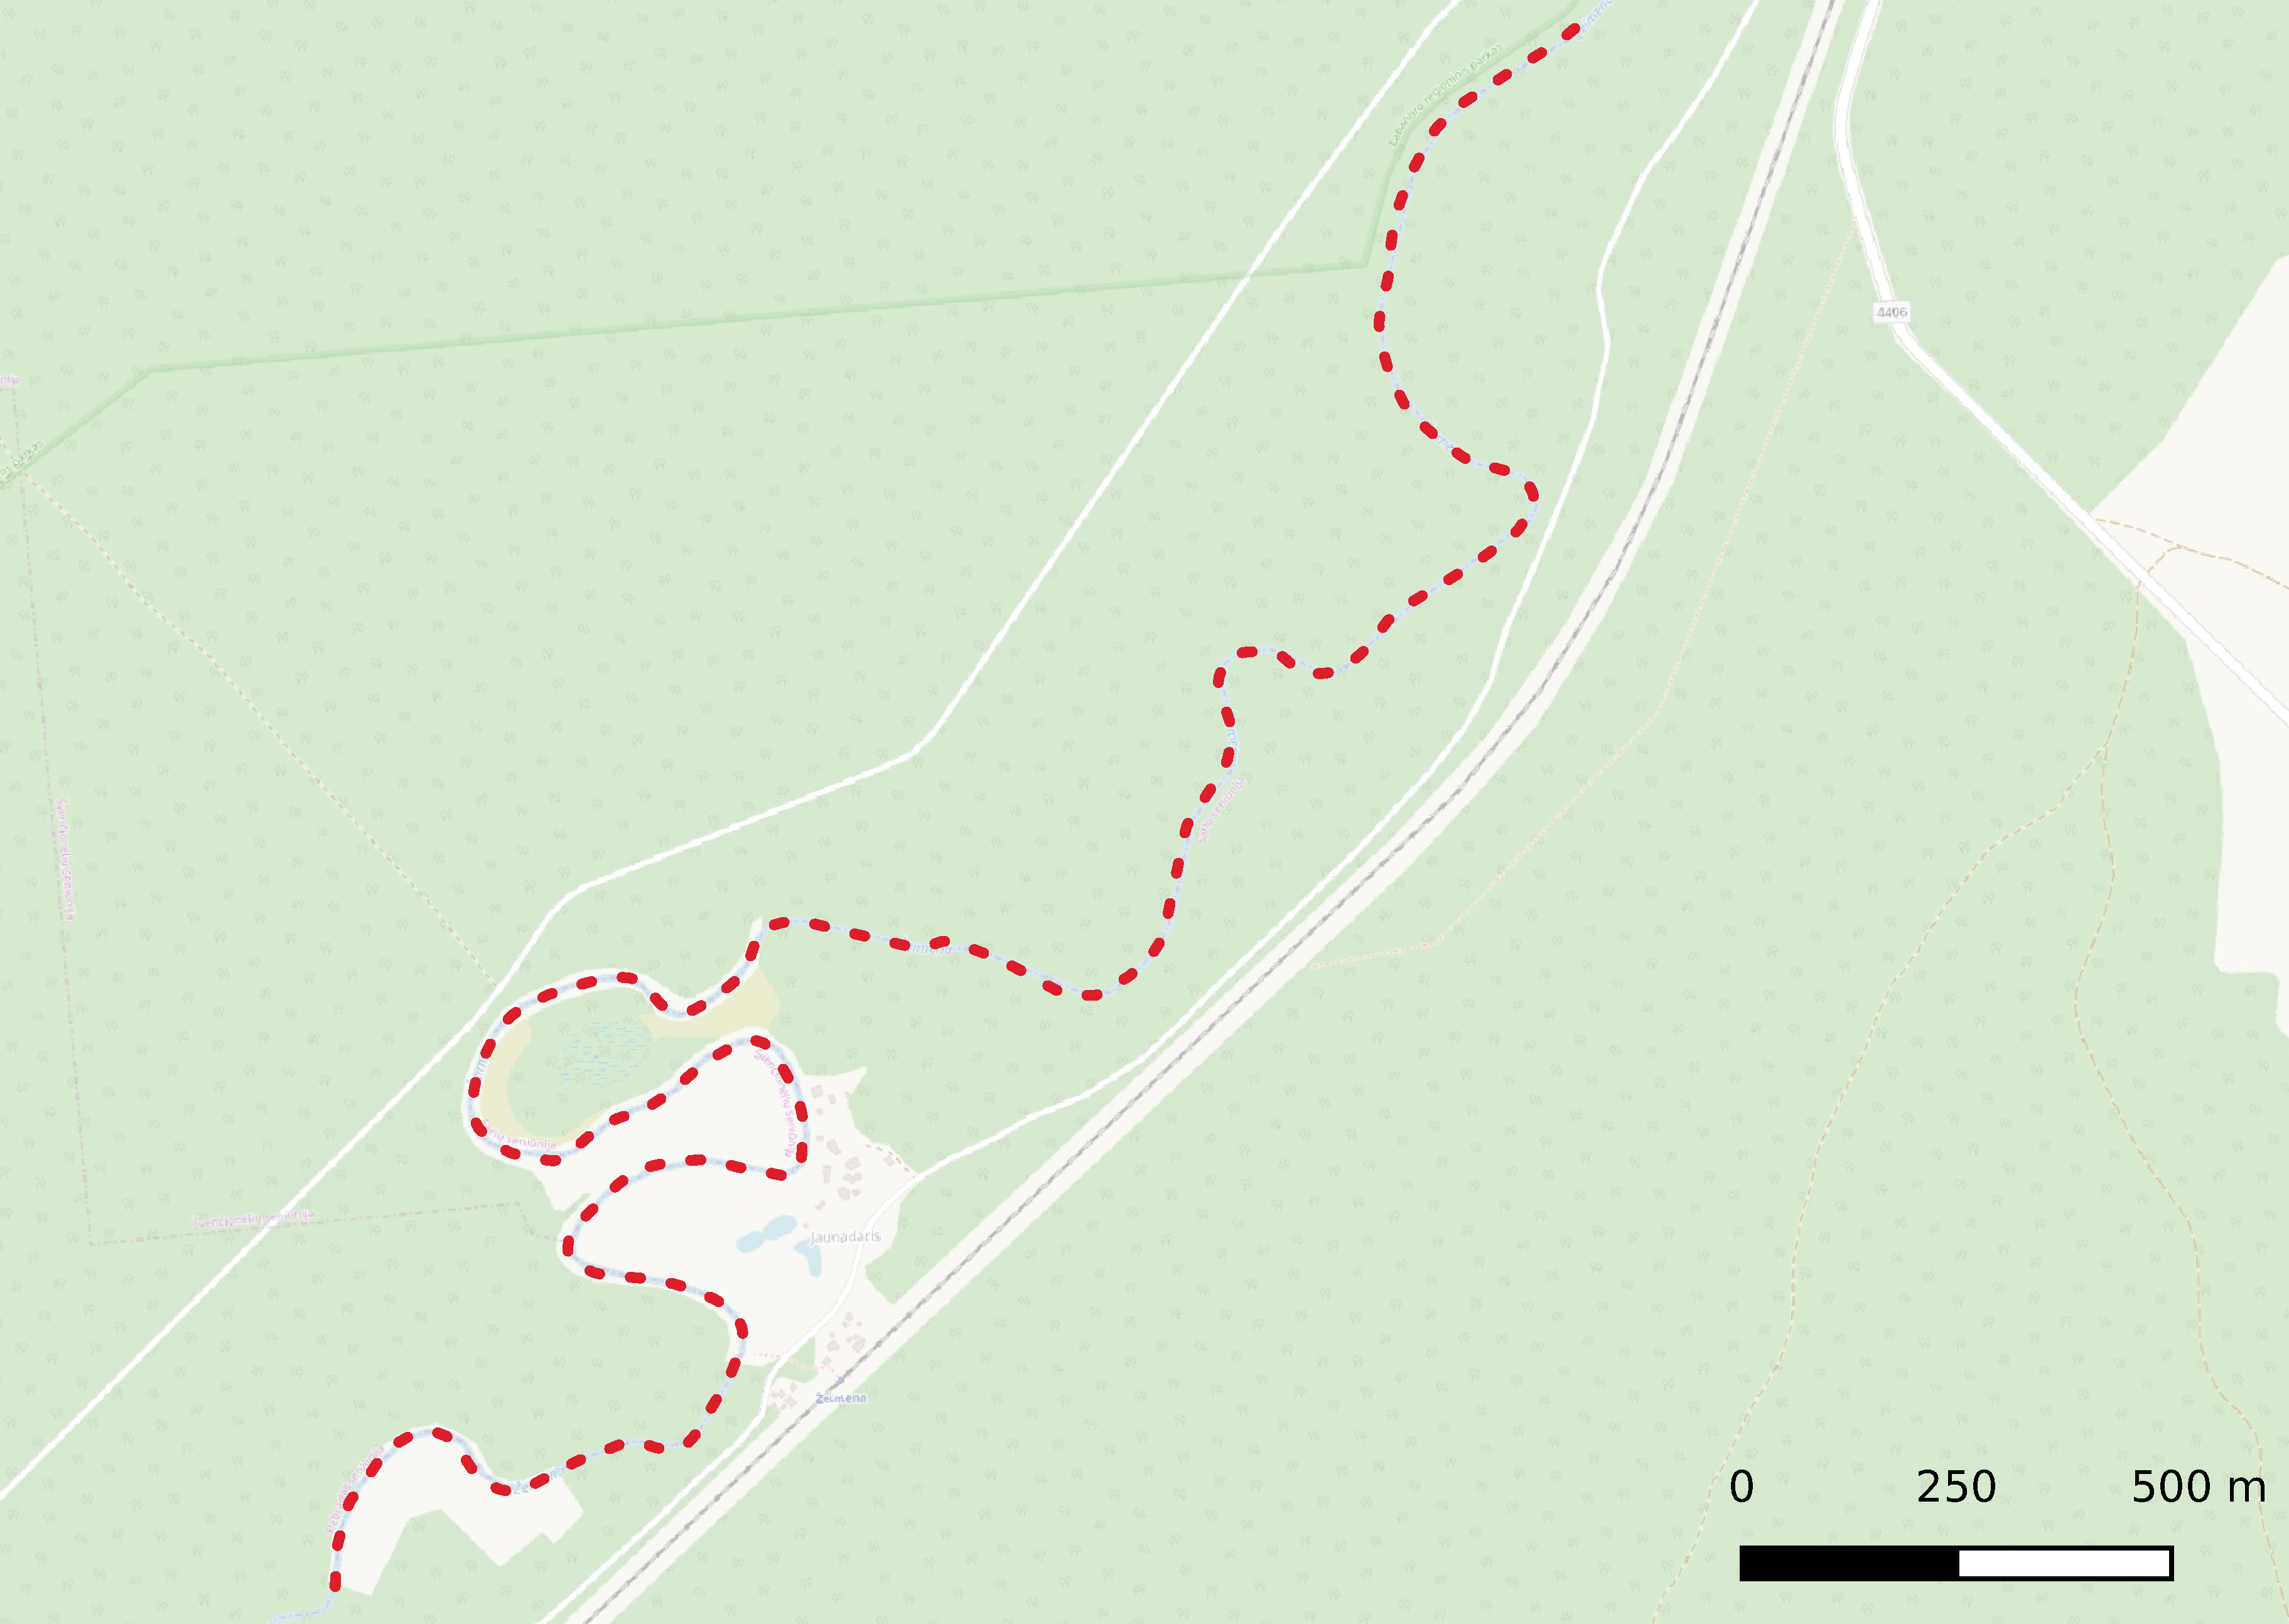
\includegraphics[width=67.5mm]{zeimena}
    \caption{Lakaja and Žeimena, $1:300000$}
    \label{fig:zeimena}
\end{figure}

\begin{figure}[h]
    \centering
    \includegraphics[width=74mm]{crossing}
    \caption{River crossing zoomed in, $1:30000$}
    \label{fig:crossing}
\end{figure}


To visually evaluate the Žeimena sample, examples for {\DP} and {\VW}
were created using the following parameters:

\begin{enumerate}[label=(\Roman*)]
    \item {\DP} tolerance: $tolerance := 125 * 2^n, n = 0,1,...,5$.
    \item {\VW} tolerance: $vwtolerance = tolerance ^ 2$\label{itm:2}.
\end{enumerate}

Parameter~\ref{itm:2} requires explanation. Tolerance for {\DP} is specified in
linear units, in this case, meters. Tolerance for {\VW} is specified in area
units $m^2$. As author was not able to locate formal comparisons between the
two (i.e. how to calculate one tolerance value from the other, so the results
are comparable?), {\DP} tolerance was arbitrarily squared and fed to {\VW}. To
author's eye, this provides comparable and reasonable results, though could be
researched.

As can be observed in table~\ref{tab:comparison-zeimena} on
page~\pageref{tab:comparison-zeimena}, both simplication algorithms convert
bends to chopped lines. This is especially visible in tolerances 250 and 500.
In a more robust simplification algorithm, the larger tolerance, the larger the
bends on the original map should be retained.

\begin{figure}[h]
    \renewcommand{\tabularxcolumn}[1]{>{\center\small}m{#1}}
    \begin{tabularx}{\textwidth}{ p{2.1cm} | X | X | }
        Tolerance DP/VW                                                   &
        Douglas \& Peucker                                                &
        Visvalingam-Whyatt                                                \tabularnewline \hline

        125/15625                                                         &
        \includegraphics[width=\linewidth]{zeimena-douglas-125}           &
        \includegraphics[width=\linewidth]{zeimena-visvalingam-125}       \tabularnewline \hline

        250/62500                                                         &
        \includegraphics[width=.5\linewidth]{zeimena-douglas-250}         &
        \includegraphics[width=.5\linewidth]{zeimena-visvalingam-250}     \tabularnewline \hline

        500/250000                                                        &
        \includegraphics[width=.25\linewidth]{zeimena-douglas-500}        &
        \includegraphics[width=.25\linewidth]{zeimena-visvalingam-500}    \tabularnewline \hline

        1000/1000000                                                      &
        \includegraphics[width=.125\linewidth]{zeimena-douglas-1000}      &
        \includegraphics[width=.125\linewidth]{zeimena-visvalingam-1000}  \tabularnewline \hline

        2000/4000000                                                      &
        \includegraphics[width=.0625\linewidth]{zeimena-douglas-2000}     &
        \includegraphics[width=.0625\linewidth]{zeimena-visvalingam-2000} \tabularnewline \hline

        4000/16000000                                                     &
        \includegraphics[width=.0625\linewidth]{zeimena-douglas-4000}     &
        \includegraphics[width=.0625\linewidth]{zeimena-visvalingam-4000} \tabularnewline \hline
    \end{tabularx}
    \caption{{\DP} and {\VW} on Žeimena}
    \label{tab:comparison-zeimena}
\end{figure}


To sum up, both {\VW} and {\DP} simplify the lines, but their cartographic
output poorly represents lines and bends. Where to look for better output?

\subsection{Combining bends}

Consecutive small bends should be combined into larger bends, and that is one
of the least developed aspects of automatic line generalization, according to
\cite{miuller1995generalization}. {\WM} encoded this process to an algorithm.

Imagine there are two small bends close to each other, similar to
figure~\ref{pic:sinewave} on page~\pageref{pic:sinewave}, and one needs
to generalize it. The bends are too large to ignore replace them with a
straight line, but too small to retain both and retain their complexity.

\begin{figure}[h]
    \centering
    \includegraphics[width=52mm]{sinewave}
    \caption{Example river bend that should be generalized}
    \label{pic:sinewave}
\end{figure}

When one applies {\DP} to figure~\ref{pic:sinewave}, either both bends remain,
or become a straight line, see table~\ref{tab:comparison-sinewave} on
page~\pageref{tab:comparison-sinewave}.

\begin{figure}[h]
    \renewcommand{\tabularxcolumn}[1]{>{\center\small}m{#1}}
    \begin{tabularx}{\textwidth}{ p{1.5cm} | X | X | }
        Tolerance DP/VW                                             &
        Douglas \& Peucker                                          &
        Visvalingam-Whyatt                                          \tabularnewline \hline

        1/1                                                         &
        \includegraphics[width=\linewidth]{sinewave-douglas-1}      &
        \includegraphics[width=\linewidth]{sinewave-visvalingam-1}  \tabularnewline \hline

        20/400                                                      &
        \includegraphics[width=\linewidth]{sinewave-douglas-20}     &
        \includegraphics[width=\linewidth]{sinewave-visvalingam-20} \tabularnewline \hline

        30/900                                                      &
        \includegraphics[width=\linewidth]{sinewave-douglas-30}     &
        \includegraphics[width=\linewidth]{sinewave-visvalingam-30} \tabularnewline \hline

        40/1600                                                     &
        \includegraphics[width=\linewidth]{sinewave-douglas-40}     &
        \includegraphics[width=\linewidth]{sinewave-visvalingam-40} \tabularnewline \hline

    \end{tabularx}
    \caption{{\DP} and {\VW} on example wave}
    \label{tab:comparison-sinewave}
\end{figure}

\section{Related Work and future suggestions}
\label{sec:related_work}

\cite{stanislawski2012automated} studied different types of metric assessments,
such as Hausdorff distance, segment length, vector shift, surface displacement,
and tortuosity for the generalization of linear geographic elements. This
research can provide references to the appropriate settings of the line
generalization parameters for the maps at various scales.

As noted in parameter~\ref{itm:2} on page~\pageref{itm:2}, it would be useful
to have a formula mapping {\DP} tolerance to {\VW}. That way, visual
comparisons between line simplification algorithms could be more objective.

\section{Conclusions}
\label{sec:conclusions}

We have practically evaluated two readily available line simplification
algorithms with a river sample: {\VW} and {\DP}, and outlined their
deficiencies. We are suggesting to implement {\WM} and compare it to the other
two.

\printbibliography

\begin{appendices}

\begin{figure}[H]
    \centering
    \includegraphics[width=148mm]{zeimena-pretty}
    \caption{Lakaja and Žeimena river in context}
\end{figure}

\end{appendices}

\end{document}
